\documentclass{article}
\usepackage[utf8]{inputenc}
\usepackage[czech]{babel}
\usepackage{syntax}
\usepackage{graphicx}
\usepackage{minted}

\hyphenpenalty 10000
\exhyphenpenalty 10000
% \usepgfplotslibrary{external}
% \tikzexternalize
\usepackage[pdftex]{hyperref}
\usepackage{url}
\DeclareUrlCommand\url{\def\UrlLeft{<}\def\UrlRight{>} \urlstyle{tt}}
\hypersetup{colorlinks=true,
  unicode=true,
  linkcolor=black,
  citecolor=black,
  urlcolor=black,
  bookmarksopen=true}

\begin{document}

\begin{titlepage}
   \begin{center}
       \vspace*{1cm}
        \Huge
       % \textbf{Cvičení 5}

       \vspace{0.5cm}
        Komplexní IR systém\
        
        KIV/IR
            
       \vspace{1.5cm}

       \textbf{David Markov}

       \vfill
            
            
       \vspace{0.8cm}
     
       %\includegraphics[width=0.4\textwidth]{university}
            
       Fakulta aplikovaných věd\\
       Západočeská univerzita v Plzni\\
       \today
            
   \end{center}
\end{titlepage}

\tableofcontents
\thispagestyle{empty}
\newpage
\setcounter{page}{1}

\section{Zadání}
Cílem semestrální práce je naučit se implementovat komplexní IR systém s využitím hotových knihoven pro preprocessing. Vedlejším produktem bude hlubší porozumění indexerům, vyhledávacím systémům a přednáškám.

Systém po předchozím předzpracování zaindexuje zadané dokumenty a poté umožní vyhledávání nad vytvořeným indexem. Vyhledávání je možné zadáním dotazu s logickými operátory AND, OR, NOT a s použitím závorek. Výsledek dotazu by měl vrátit top x (např. 10) relevantních dokumentů seřazených dle relevance.


Minimální nutná funkčnost semestrání práce pro získání 15 bodů (a tedy potenciálně zápočtu):

Tokenizace, preprocessing (stopwords remover, stemmer/lemmatizer), \newline vytvoření in-memory invertovaného indexu, tf-idf model, cosine similarity, \newline vyhledávání dotazem vrací top x výsledků seřazených dle relevance (tj. vektorový model - vector space model), vyhledávání logickými operátory AND, OR, NOT (booleovský model), podrobná dokumentace (programátorská i uživatelská), podpora závorek pro vynucení priority operátorů.

Semestrální práce musí umožňovat zaindexování dat stažených na cvičení (1. bodované cvičení Crawler) a libovolných dalších dat ve stejném formátu. Obě sady dat je možné zaindexovat nezávisle na sobě.

Semestrální práce musí umožňovat zadávat dotazy z GUI nebo CLI (command line interface) a při zadávání dotazů je možno vybrat index a model vyhledávání (vector space model vs. boolean model). Výsledky vyhledávání obsahují i celkový počet dokumentů, které odpovídají zadanému dotazu.

 

Nadstandardní funkčnost (lze získat až dalších 15 bodů), např.:
\begin{itemize}
    \item File-based index
    \item Pozdější doindexování dat - přidání nových dat do existujícího indexu
    \item Ošetření HTML tagů
    \item Detekce jazyka dotazu a indexovaných dokumentů
    \item Vylepšení vyhledávání
    \item Vyhledávání frází (i stop slova)
    \item Vyhledávání v okolí slova
    \item Více scoring modelů
    \item Indexování webového obsahu - zadám web, program stáhne data a rovnou je zaindexuje do existujícího indexu
    \item Další předzpracování normalizace
    \item GUI/webové rozhraní
    \item Napovídání keywords
    \item Podpora více polí pro dokument (např. datum, od do)
    \item Zvýraznění hledaného textu v náhledu výsledků
    \item Vlastní implementace parsování dotazů bez použití externí knihovny
    \item Implementace dalšího modelu (použití sémantických prostorů, doc2vec, Transformers - BERT) atd.
\end{itemize}

\section{Popis implementovaného systému}
V rámci semestrální práce byl vyvinut systém pro vyhledávání a indexaci dokumentů. Aplikace uživateli umožňuje vyhledávat v zaindexovaných dokumentech pomocí řetězcových dotazů z uživatelského rozhraní. Výsledky vyhledávání jsou uživateli následně kompaktně zobrazovány. 

Systém navíc umožňuje spuštění bez přidaných vlastních dat, kdy si sám vyhledá data z odpovídajícího webu a automaticky je zaindexuje ihned po startu.

\subsection{Uživatelská příručka}
Pro spuštění aplikace je třeba mít nastaven pracovní adresář jako kořenový adresář projektu a z terminálu spustit následující:

\begin{minted}{bash}
    java -jar search-engine.jar [-OPTION]
\end{minted}

Při spuštění systému z příkazové řádky je možné předávat následující parametry:
\begin{itemize}
    \item \texttt{-h (--help)} - vypíše nápovědu
    \item \texttt{-s (--storage) <memory/file>} - specifikuje implementaci úložiště dokumentů k pozdějšímu zaindexování - v paměti nebo na disku (výchozí variantou je implementace diskového úložiště)
        \begin{itemize}
            \item POZNÁMKA: paměťová implementace úložiště dokumentů je určena pouze pro účely vývoje a neměla by se využívat při reálném běhu aplikace; aktuálně není toto úložiště podporováno a jeho volba ukončí systém výjimkou jelikož některé operace rozhraní úložiště nejsou momentálně podporovány
        \end{itemize}
\end{itemize}

Požadavkem pro spuštění předem sestaveného spustitelného souboru je nainstalovaný \textit{Java Runtime Environment (JRE) 17} nebo novější.

\newpage
Po spuštění může uživatel se systémem interagovat pomocí uživatelského rozhraní a ovládat tak vyhledávací engine. Podporované příkazy jsou:
\begin{itemize}
    \item \texttt{clear} - vyčistí obrazovku terminálu
    \item \texttt{exit} - korektně ukončí aplikaci
    \item \texttt{query <query string> [--model <boolean/vector]} - vyhledá v indexu dokumenty, které odpovídají zadanému dotazu
    \begin{itemize}
        \item volitelným parametrem \texttt{--model} lze specifikovat jaký vyhledávací model se má při vyhledávání použít; aktuálně podporovanými variantami jsou \textit{Booleovský model} a \textit{Vektorový model}, přičemž vektorový model je výchozí variantou
    \end{itemize}
    \item \texttt{url <url>} - vyhledá zadanou URL (musí být absolutní z \url{https://hokej.cz} nebo relativní), ze které zpracuje článek; zpracovaný článek je uložen do úložiště dokumentů a je zaindexován při dalším spuštění aplikace
\end{itemize}

Po zadání dotazu jsou vyhledány odpovídající dokumenty v indexu a jsou kompaktně prezentovány na uživatelském rozhraní. Uveden je použitý vyhledávací model, počet nalezených dokumentů a u každého nalezeného dokumentu je uvedeno jeho celočíselné ID, skóre, titulek, autor článku, datum publikace a krátký úryvek ze začátku obsahu. Seznam vyhledaných výsledků je navíc seřazen podle skóre sestupně (viz obr. \ref{fig:ui}).

\begin{figure}[!h]
    \centering
    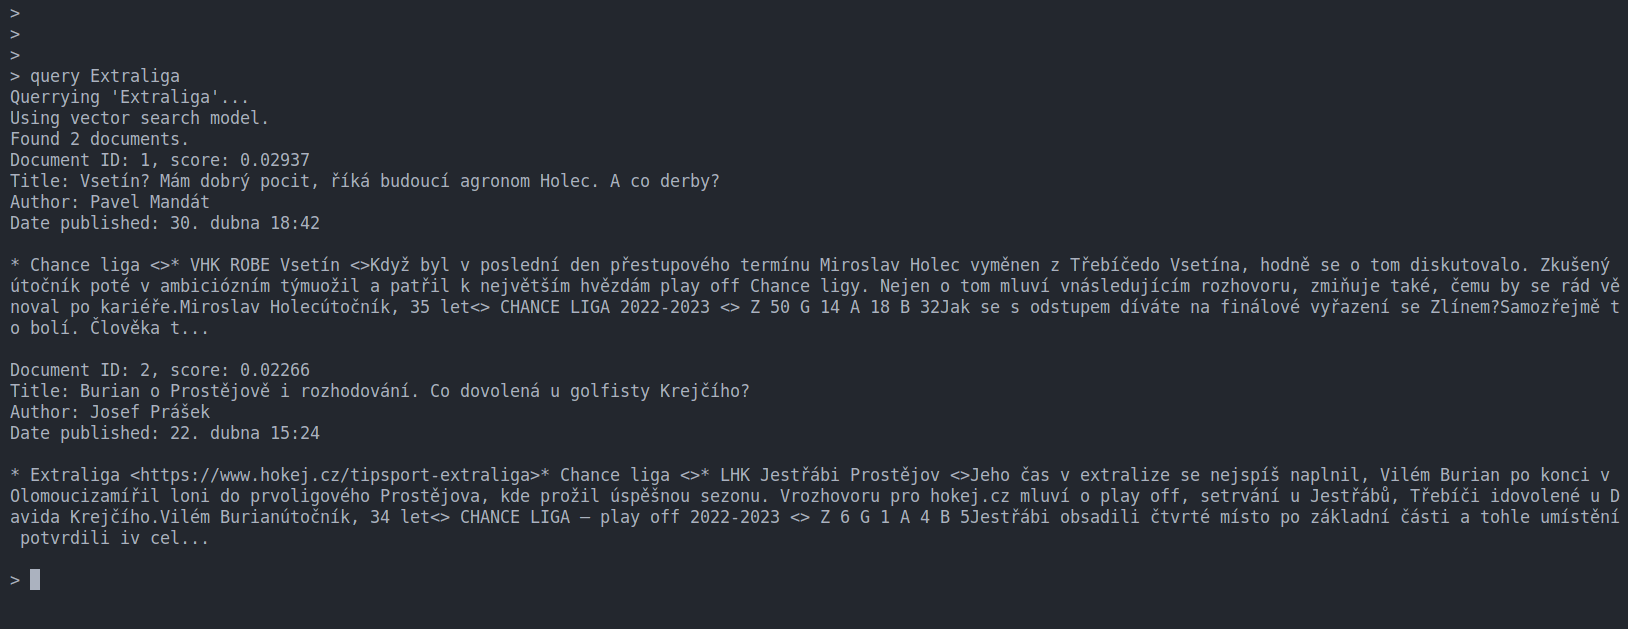
\includegraphics[width=\columnwidth]{img/UI.png}
    \caption{Uživatelské rozhraní systému, prezentující výsledky vyhledávání.}
    \label{fig:ui}
\end{figure}

\newpage
\subsection{Sestavení systému z přiložených zdrojových souborů}
Spustitelný soubor systému je samozřejmě možné snadno sestavit z přiložených zdrojových souborů. Stačí jednoduše nastavit pracovní adresář jako kořenový adresář projektu a z terminálu spustit příkaz 

\begin{minted}{bash}
    mvn clean package
\end{minted}

Tento příkaz sestaví všechny \textit{Maven} moduly systému a vytvoří spustitelný \texttt{.jar} soubor v adresáři \texttt{core/target} s názvem \newline \texttt{search-engine-<verze>-jar-with-dependencies.jar}. Ten je následně možné spustit stejným způsobem, jak již bylo zmíněno dříve.

Požadavky pro sestavení ze zdrojových souborů jsou nainstalované programy \textit{Maven} a \textit{Java Development Kit (JDK) 17} nebo novější.

\subsection{Indexace vlastních dokumentů}
Systém umožňuje snadno indexovat své vlastní dokumenty, které odpovídají očekávanému formátu. Jednoduše stačí dokumenty přidat do adresáře úložistě dokumentů \texttt{storage} a při dalším spuštění budou zaindexovány. Pokud soubor nebude odpovídat předpokládanému formátu, bude zalogována chyba a přejde se na načtení dalšího souboru.

\section{Detaily implementace}
Spuštění systému je provedeno v několika po sobě jdoucích krocích.

Nejprve se zkontroluje přítomnost zaindexovaných dat v indexu. Pokud jsou nalezena zaindexovaná data, je uživateli ihned prezentováno uživatelské rozhraní. Je třeba zmínit, že tento krok byl přidám primárně pro účely implementace indexu v souboru, který uchovává data napříč jednotlivými běhy systému. Jelikož je podporován pouze paměťový, data nebudou při startu nikdy nalezena a spouštění postoupí do druhé fáze.

Ve druhém kroku je zkontrolována přítomnost dat v úložišti dokumentů k indexaci v adresáři \texttt{storage}. Pokud jsou uloženy záznamy k indexaci, jsou objektem \texttt{Storage} načteny do paměti a zaindexovány. Pokud v úložišti nejsou žádné záznamy, spouštění postoupí do třetího kroku.

V tomto kroku následuje kontrola úložiště URL adres článků ke zpracování Crawlerem, uchování článků do úložiště a jejich následná indexace. Procházení potřebného webu a zpracování jednotlivých článků je časově náročné a proto je implementován mezikrok, ve kterém jsou tyto články založeny do úložiště. To umožňuje výrazně urychlit budoucí běhy vyhledávacího enginu, jelikož nemusí články neustále zpracovávat.

Pokud nejsou přítomny ani uložené URL adresy jednotlivých článků, je nejprve zpracována domovská stránka webu \url{https://hokej.cz}, ze které jsou načteny všechny potřebné URL a jsou přidány do úložiště, aby je nebylo nutné znovu načítat v příštím běhu. Celý proces je znázorněn v sekvenčním diagramu na obrázku \ref{fig:startup-sequence-diagram}.

\begin{figure}
    \centering
    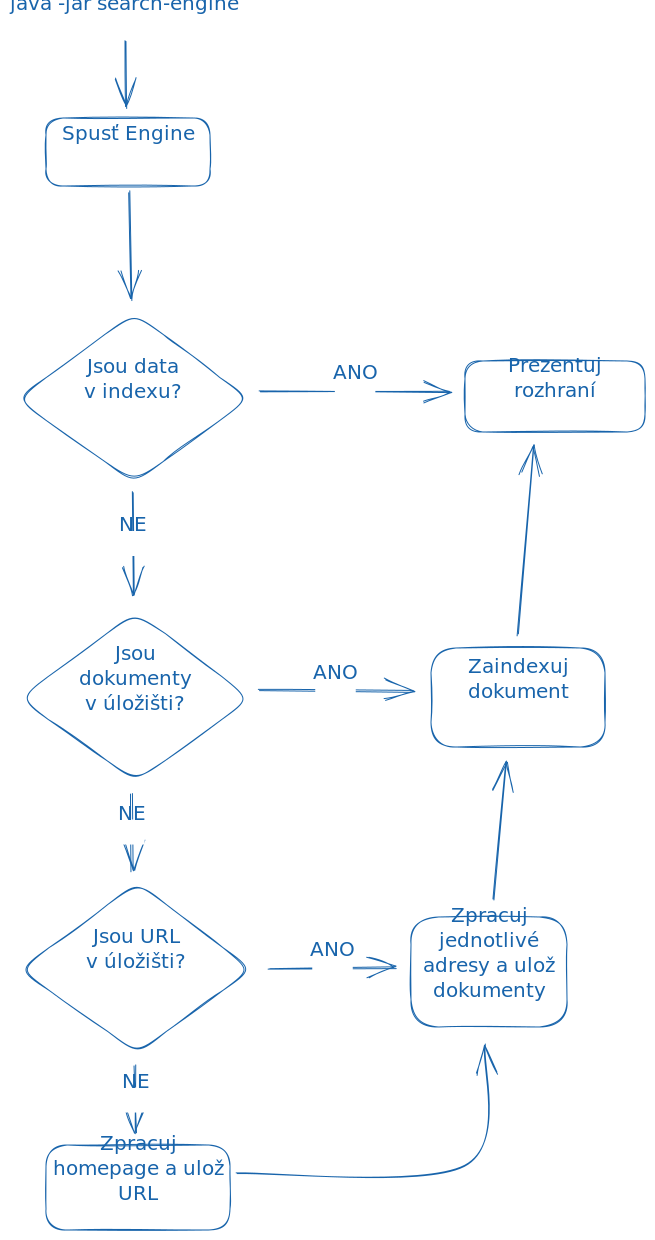
\includegraphics[width=0.7\columnwidth]{img/sequence-diagram.png}
    \caption{Sekvenční diagram, popisující kroky spuštění systému.}
    \label{fig:startup-sequence-diagram}
\end{figure}

\subsection{Moduly systému}
Systém je rozdělen do dvou samostatných modulů, na kterých je dále závislý modul jádra systému.

\paragraph{Search Engine Utilities} je modul, obsahující pomocné metody a funkce, které je možné využít napříč širokou škálou systémů. Jsou to například pomocné funkce pro práci se soubory, řetězci či URL odkazy. Dále jsou zde implementovány třídy, specifické pro tento systém, které mohou být dále využity v dalších modulech systému. Těmi jsou například třída \textit{Storage}, zodpovědná za správu úložiště dokumentů pro indexaci nebo \textit{FileLoader}, který poskytuje rozhraní pro načítání objektů ze souborů.

\paragraph{Search Engine Crawler} obsahuje veškerou logiku, potřebnou k procházení webu, zpracování webových stránek a získávání potřebných dat z jednotlivých článků. Základem celého modulu je třída \textit{Crawler}, která pro všechny tyto operace poskytuje rozhraní. Modul je závislý na již zmíněném modulu \texttt{utils}, jelikož využívá například třídu \textit{Storage} k ukládání obsahu zpracovaných článků z webu do úložiště.

\paragraph{Search Engine Core} je nosným prvkem celého systému. Obsahuje logiku spouštění aplikace, uživatelské rozhraní, které zpracovává požadavky uživatele, implementaci indexu pro vyhledávání dokumentů i parser jednotlivých dotazů do indexu. Spojuje celý systém do jednoho celistvého programu a je závislý na všech ostatních samostatných modulech projektu. Pro indexaci dokumentů poskytuje rozhraní \textit{Index} a jeho implementaci \textit{TfIdfIndex}, která pro indexování a vážení jednotlivých dokumentů a slov používá výpočet \textit{TF-IDF}.

\paragraph{Logování} v celém systému je zajištěno knihovnou \textit{SLF4J}. Všechny logy jsou zaznamenávány na různých úrovních detailu do souboru v adresáři \texttt{logs}. Zde jsou logy uchovávany po jeden den, poté jsou přeměněny do komprimované podoby pro pozdější využití.

\section{Implementovaná nadstandardní funkčnost}
Zde je uveden seznam nadstandardních implementovaných funkčností oproti základnímu zadání:
\begin{itemize}
    \item Česká dokumentace v TeXu a anglické README v Markdownu 
    \item Systém logování s následnou komprimací záznamů po uplynutí časového intervalu.
    \item Modularizace projektu do dílčích \textit{Maven} modulů
    \item Snadno rozšiřitelná parametrizace spouštění systému pomocí přepínačů
    \item Cache jednotlivých kroků při startu systému
    \item Integrace web-crawleru do systému
    \item Crawlování zadané URL adresy a získání článku, který je později zaindexován
\end{itemize}

\section{Výsledky TREC evaluace}
Při evaluaci třídou \textit{TestTrecEval.java} bylo dosaženo následujících výsledků:
\begin{itemize}
    \item \textit{MAP} při vyhledání pomocí \texttt{Topic::getTitle} - \(0.1074\)
    \item \textit{MAP} při vyhledání pomocí \texttt{Topic::getNarrative} - \(0.1004\)
    \item \textit{MAP} při vyhledání pomocí \texttt{Topic::getDescription} - \(0.1085\)
    \item \textit{MAP} pri vyhledání spojením \texttt{Topic::getTitle} a \texttt{Topic::getNarative} - \(0.1348\)
    \item \textit{MAP} pri vyhledání spojením \texttt{Topic::getTitle} a \texttt{Topic::getDescription} - \(0.1173\)
\end{itemize}

Nejlepší výsledek tedy dosáhla evaluace vyhledáváním \texttt{Topic::getTitle} a \texttt{Topic::getNarrative}. Celý výstup lze vidět na obrázku \ref{fig:trec-eval}.

\begin{figure}[!h]
    \centering
    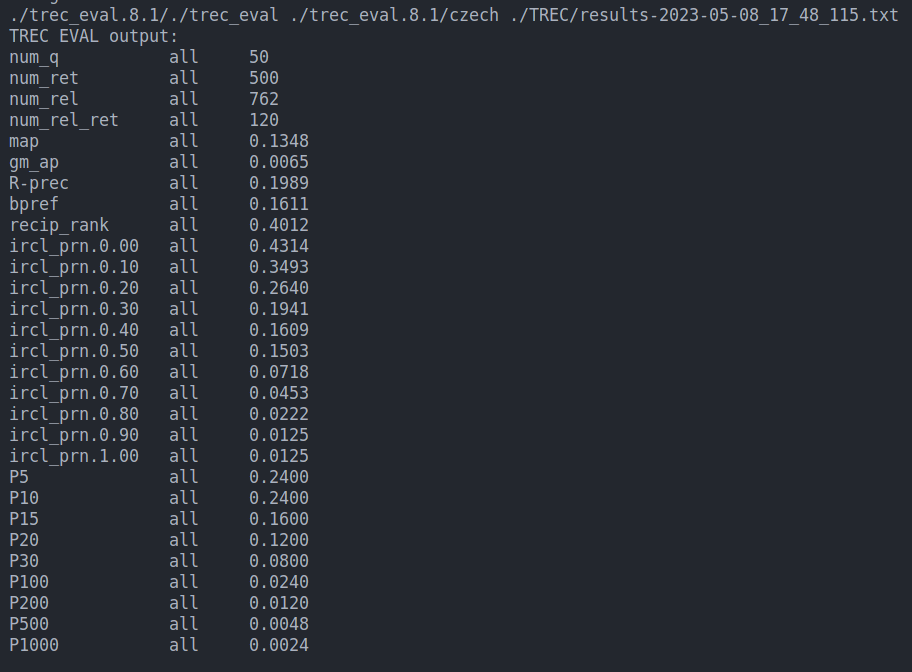
\includegraphics[width=\columnwidth]{img/trec-eval.png}
    \caption{Výsledek evaluace nad sadou dokumentů TREC s použitím \texttt{Topic::getTitle} a \texttt{Topic::getNarrative} jako dotazu.}
    \label{fig:trec-eval}
\end{figure}

\end{document}
